\documentclass[12pt,a4paper]{article}
\usepackage[utf8]{inputenc}
\usepackage[czech]{babel}
\usepackage[T1]{fontenc}
\usepackage{amsmath}
\usepackage{amsfonts}
\usepackage{amssymb}
\usepackage{graphicx}
\usepackage{titlesec}
\usepackage[left=2cm,right=2cm,top=2cm,bottom=2cm]{geometry}
\usepackage{indentfirst}
\usepackage{listings}
\usepackage{color}
\usepackage{array}
\usepackage{csquotes}
\usepackage{url}

%Pravidlo pro řádkování
\renewcommand{\baselinestretch}{1.5}

%Pravidlo pro začínání kapitol na novém řádku
\let\oldsection\section
\renewcommand\section{\clearpage\oldsection}

%Formáty písem pro nadpisy (-změněno na bezpatkové \sffamily z původního \normalfont
\titleformat{\section}
{\sffamily\Large\bfseries}{\thesection}{1em}{}
\titleformat{\subsection}
{\sffamily\large\bfseries}{\thesubsection}{1em}{}
\titleformat{\subsubsection}
{\sffamily\normalsize\bfseries}{\thesubsubsection}{1em}{}

%Nastavení zvýrazňování kódu v \lslisting
\definecolor{mygreen}{rgb}{0,0.6,0}
\definecolor{mygray}{rgb}{0.5,0.5,0.5}
\lstset{commentstyle=\color{mygreen},keywordstyle=\color{blue},numberstyle=\tiny\color{mygray}}

\author{Jan Šmejkal}

\begin{document}

%-------------Úvodni strana---------------
\begin{titlepage}


\includegraphics[width=50mm]{img/FAV.jpg}
\\[160 pt]
\centerline{ \Huge \sc KIV/BIT - Bezpečnost}
\centerline{ \Huge \sc v informačních technologiích}
\\[6 pt]
\centerline{ \LARGE \sc Semestrální práce}
\\[12 pt]
\centerline{ \large \sc Java implementace šifry}
\centerline{ \large \sc International Data Encryption Standard}


{
\vfill 
\parindent=0cm
\textbf{Jméno:} Štěpán Ševčík\\
\textbf{Osobní číslo:} A13B0443P\\
\textbf{E-mail:} kiwi@students.zcu.cz\\
\textbf{Datum:} {\large \today\par} %datum
\textbf{Celková doba řešení:} {\large $\pm 18h$} %datum

}

\end{titlepage}

%------------------------------------------

%------------------Obsah-------------------
\newpage
\setcounter{page}{2}
\setcounter{tocdepth}{3}
\tableofcontents
%------------------------------------------

%--------------Text dokumentu--------------


\section{International Data Encryption Algorithm}
Algoritmus šifrování International Data Encryption Algorithm, zkráceně IDEA, je symetrické blokové šifrování binárních dat.
IDEA je nástupce algoritmu Data Encryption Standard \cite{wiki.IDEA}. IDEA byl vyvinut ve Švýcarsku a patentován až do roku 2012, kdy vypršel poslední patent \cite{source-code.IDEA}.

\subsection{Analýza}
\begin{figure}[h]
	\centering
	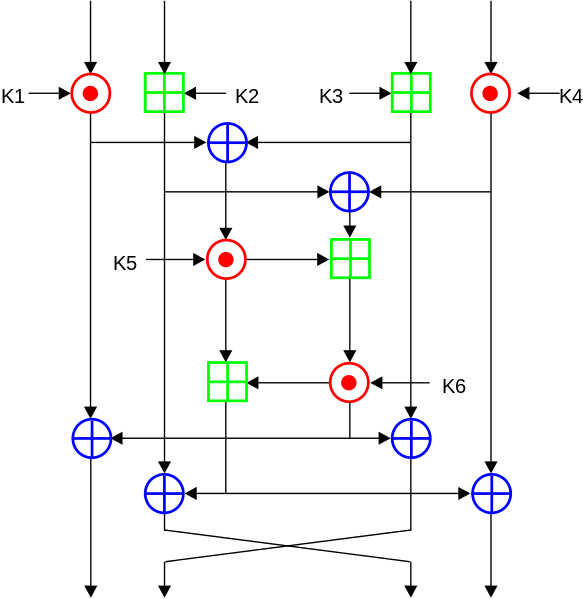
\includegraphics[width=0.4\linewidth]{img/fig_idea-step.png}
	\caption{Schéma šifrovacího kroku \cite{wiki.IDEA}}
	\label{fig:idea-step}
\end{figure}

IDEA pracuje s bloky dat o délce 64b a s klíčem délky 128b. Šifrování každého bloku dat se skládá z osmi iterací šifrovacího kroku a z výstupní transformace.
Každý blok dat je na čtyři části o velikosti 16b a zašifrován osmi iteracemi transformací znázorněných ve schématu znázorněném na Obrázku \ref{fig:idea-step}. Po aplikování iterací šifrovacího kroku je na jejich výstup použita výstupní transformace znázorněná Obrázkem \ref{fig:idea-half-step}.

\begin{figure}[h]
	\centering
	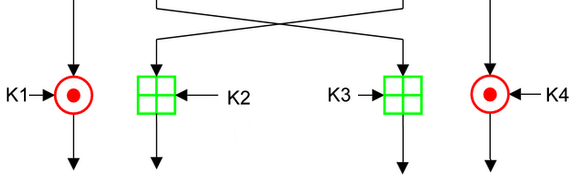
\includegraphics[width=0.4\linewidth]{img/fig_idea-half-step.png}
	\caption{Schéma výstupní transformace \cite{wiki.IDEA}}
	\label{fig:idea-half-step}
\end{figure}


\subsection{Implementace řešení}

\subsubsection{Rozhraní příkazové řádky}

\section{Uživatelská dokumentace}

\section{Závěr}

\bibliographystyle{abbrv}
{\raggedright\small
	\bibliography{literatura}
}

%------------------------------------------

\end{document}
